\documentclass[tikz, margin=2mm]{standalone}
\usepackage[sfdefault,light]{roboto}
\usetikzlibrary{
	arrows,
	arrows.meta,
	chains,
	positioning,
	shapes,
	shapes.multipart,
	mindmap,
	fit,
	calc,
	intersections,
	backgrounds,
	scopes,
	matrix,
	shadows,
}
\definecolor{MyGreen}{HTML}{41B3A3}
\definecolor{MyOrange}{HTML}{E27D60}

\tikzset{every picture/.style={/utils/exec={\sffamily}}}
\begin{document}
    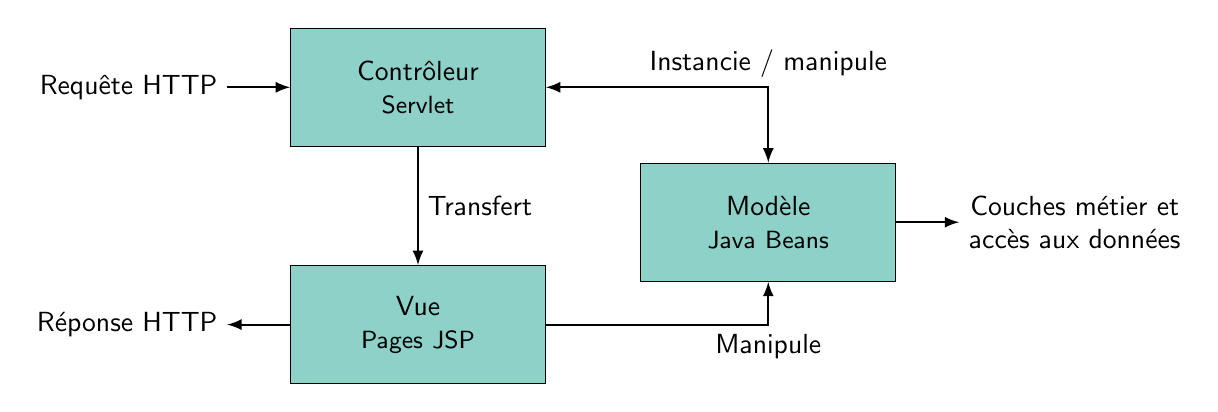
\begin{tikzpicture} [
			every node/.style={align=center,rectangle},
			comp/.style={draw,fill=MyGreen!60,minimum width=30mm,minimum height=15mm,text width=30mm}
		]	
		
		\node [comp] (controller) {
			Contrôleur \\ 
			\small Servlet
		};
		\node [comp, below=1.5cm of controller] (view) {
			Vue \\ 
			\small Pages JSP
		};
	
		\node [comp, below right=.2cm and 1.2cm of controller] (model) {
			Modèle \\ 
			\small Java Beans
		};
		\node [left=.8cm of controller] (input) {Requête HTTP};
		\node [left=.8cm of view] (output) {Réponse HTTP};
		\node [right=.8cm of model] (tier) {Couches métier et \\ accès aux données};

		\path[latex-latex,draw,thick] (controller.east) -| coordinate[midway] (cm) (model.north);
		\node[above] at (cm) {Instancie / manipule};
		\path[latex-,draw,thick] (model.south) |- coordinate[midway] (mv) (view.east);
		\node [below] at (mv) {Manipule};
		\path[-latex,draw,thick] (controller) -- coordinate[midway] (cv1) (view);
		\node [right] at (cv1) {Transfert};
		\path[-latex,draw,thick] (input) -- (controller);
		\path[latex-,draw,thick] (output) -- (view);
		\path[latex-,draw,thick] (tier) -- (model);
	\end{tikzpicture}
\end{document}